% The contents of this file is 
% Copyright (c) 2009-  Charles R. Severance, All Righs Reserved

\chapter{¿Por qué debería aprender a escribir programas?}

Escribir programas (o programar) es una actividad muy
gratificante y creativa. Puedes escribir programas por
muchas razones, desde por mantenerte activo hasta
por resolver un problema difícil de análisis de datos o
por divertirte ayudando a otros a resolver cualquier problema.
Este libro asume que \emph{todo el mundo} necesita saber programar,
y que una vez que sepas programar ya encontrarás tú mismo
la forma de aplicar tus recién adquiridas habilidades.

En nuestra vida diaria estamos rodeados de ordenadores, que van
desde portátiles hasta teléfonos móviles. Podemos pensar en esos
ordenadores como nuestros ``asistentes personales'', que pueden
ocuparse de muchas cosas por nosotros. El hardware en los equipos
que usamos a diario está creado esencialmente para hacernos
continuamente la pregunta,
``¿Qué quieres que haga a continuación?''

\beforefig
\centerline{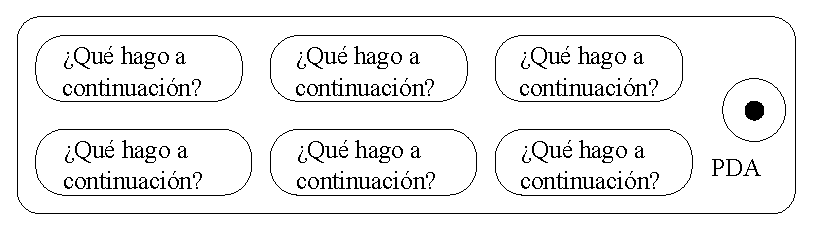
\includegraphics[height=1.00in]{figs2/pda.eps}}
\afterfig

Los programadores añaden un sistema operativo y un conjunto de
aplicaciones al hardware y así tenemos al final un Asistente Personal
Digital que resulta bastante útil y capaz de ayudarnos a hacer
muchas cosas diferentes.

Nuestros ordenadores son rápidos, tienen gran cantidad de memoria
y podrían resultarnos muy útiles si tan solo conociéramos el idioma
que debemos hablar para explicar al ordenador qué queremos que
´´haga a continuación''. Si conociéramos ese idioma, podríamos pedirle al
ordenador que realizase tareas repetitivas para nosotros. 
Precisamente, el tipo de cosas que los ordenadores hacen mejor
suelen ser el tipo de cosas que los humanos encuentran aburridas
y soporíferas.

Por ejemplo, echa un vistazo a los primeros tres párrafos de este
capítulo y dime cual es la palabra más utilizada y cuántas veces
se ha usado. A pesar de que seas capaz de leer y comprender
las palabras en unos pocos segundos, contarlas cuesta más,
porque no es el tipo de problema que las mentes humanas
fueron diseñadas para resolver. Para un ordenador
es justo al revés: leer y comprender texto
de un trozo de papel es algo complicado para él,
pero contar las palabras y decir cuántas veces
se ha usado la más frecuente le resulta muy sencillo:

\beforeverb
\begin{verbatim}
python words.py
Introduce fichero:words.txt
que 8
\end{verbatim}
\afterverb
%
Nuestro ``asistente analista de información personal'' nos dirá
rápidamente que la palabra ``que'' se ha usado ocho veces en los
primeros tres párrafos de este capítulo.

El hecho de que los ordenadores sean buenos en cosas
en las que los humanos no lo son es el motivo por el que necesitas
ser capaz de hablar ``idioma de ordenador''. Una vez que hayas
aprendido ese nuevo idioma, podrás delegar tareas mundanas
en tu socio (el ordenador), dejando más tiempo libre
para ti, de modo que puedas dedicarte a aquellas otras cosas
para las que estás más capacitado. Serás el encargado
de poner la creatividad, intuición e inventiva a esa
asociación.

\section{Creatividad y motivación}

Aunque este libro no está dirigido a programadores profesionales, la programación
profesional puede ser un trabajo muy gratificante tanto a nivel financiero como personal.
Construir programas útiles, elegantes e ingeniosos para que otros los usen
es una actividad muy creativa. Tu ordenador o Asistente Personal Digital (PDA),
normalmente contienen muchos programas diferentes de multitud de grupos de programadores
distintos, cada uno de los cuales compite por tu atención e interés.
Esos programadores intentan hacerlo lo mejor que saben para adaptarse a tus necesidades y
proporcionarte una buena experiencia de usuario en tu tarea. En algunos casos, cuando eliges un
programa determinado, los programadores son directamente recompensados por tu elección.

Si pensamos en los programas como salida creativa para grupos de programadores,
tal vez la siguiente figura sea una versión más acertada de tu PDA:

\beforefig
\centerline{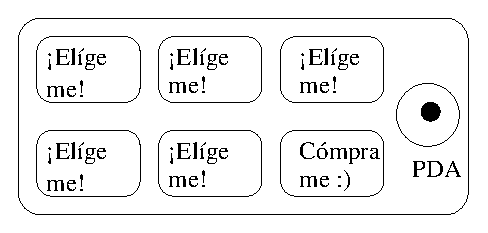
\includegraphics[height=1.00in]{figs2/pda2.eps}}
\afterfig

Por ahora, nuestra motivación principal no es conseguir dinero o gustar más a los usuarios
finales, sino ser más productivos para nosotros mismos en el manejo de los datos e
información que encontraremos en nuestras vidas.
Al principio, serás tanto programador como usuario final de tus propios programas.
Cuando ganes en habilidad como programador y la programación se haga más creativa para ti,
tus ideas podrán avanzar desarrollando programas para otros.

\section{Arquitectura hardware del ordenador}
\index{hardware}
\index{hardware!architecture}

Antes de que empecemos a aprender el idioma que deberemos hablar
para dar instrucciones a los ordenadores o desarrollar
software, necesitamos aprender un poco acerca de cómo
están construidos los ordenadores. Si desmontaras
tu ordenador o teléfono móvil y mirases dentro,
encontrarías los siguientes componentes:

\beforefig
\centerline{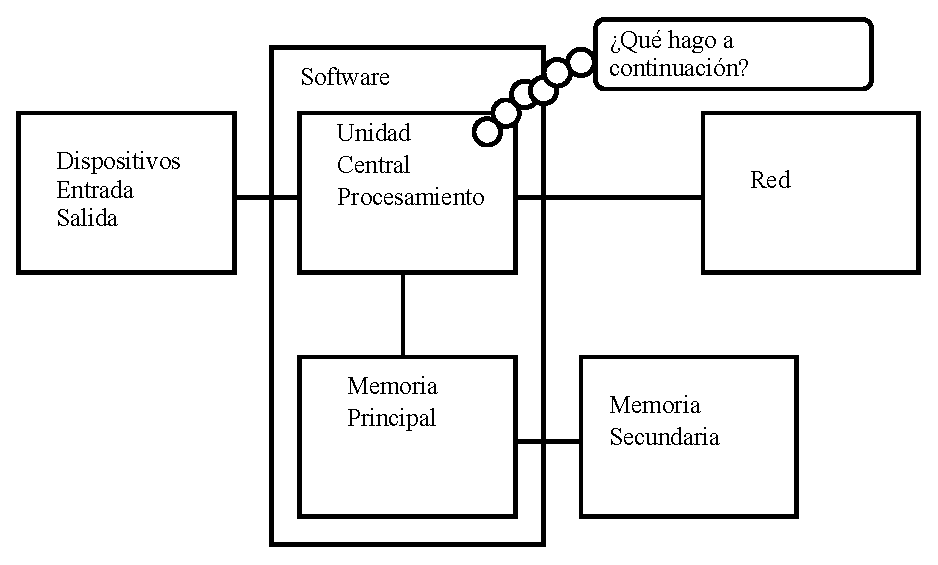
\includegraphics[height=2.50in]{figs2/arch.eps}}
\afterfig

Las definiciones de alto-nivel de estos componentes son las siguientes:

\begin{itemize}

\item La {\bf Unidad Central de Procesamiento} (o CPU) es
la parte del ordenador que está construida para estar obsesionada
con el ``¿qué es lo siguiente?'' Si tu ordenador está clasificado
como de 3.0 Gigahercios, significa que la CPU va a preguntar ``¿Qué hago a continuación?''
tres mil millones de veces por segundo. Tendrás que aprender a hablarle muy
rápido para mantener el ritmo de esa CPU.

\item La {\bf Memoria Principal} se usa para almacenar la información
que la CPU necesitará enseguida. La memoria principal es casi
tan rápida como la CPU. Pero la información almacenada en la memoria
principal se desvanece cuando el ordenador se apaga.

\item La {\bf Memoria Secundaria} Es también utilizada para almacenar
información, pero es mucho más lenta que la memoria principal.
La ventaja de la memoria secundaria es que puede mantener
almacenada la información incluso cuando el ordenador está apagado.
Ejemplos de memoria secundaria son las unidades de disco o las
memorias flash (que se encuentran normalmente en lápices USB y
reproductores de música portátiles).

\item Los {\bf Dispositivos de Entrada y Salida} son simplemente
la pantalla, teclado, ratón, micrófono, altavoces, touchpad, etc.
Son todos los aparatos que utilizamos para interactuar con el ordenador.

\item En la actualidad, la mayoría de los ordenadores disponen también de una
{\bf Conexión de Red} para recibir información a través de la red.
Podemos pensar en la red como en un sitio muy lento donde se almacenan
y recuperan datos, que puede no estar siempre ``preparado''. Así que en cierto sentido,
la red es una forma lenta y a veces poco fiable de
{\bf Memoria Secundaria}.

\end{itemize}

Aunque la mayoría de los detalles de cómo funcionan estos componentes es mejor
dejarlos para los que construyen ordenadores, resulta útil tener cierta terminología
con la que referirnos a todas estas partes distintas mientras escribimos nuestros programas.

Como programador, tu trabajo es usar y orquestar cada uno de esos
recursos para resolver el problema que necesites solucionar
y analizar los datos que obtengas de la solución. Como programador, principalmente
estarás ``hablando'' con la CPU y diciéndole qué debe hacer a continuación.
A veces le dirás a la CPU que use la memoria principal,
la memoria secundaria o los dispositivos de entrada/salida.

\beforefig
\centerline{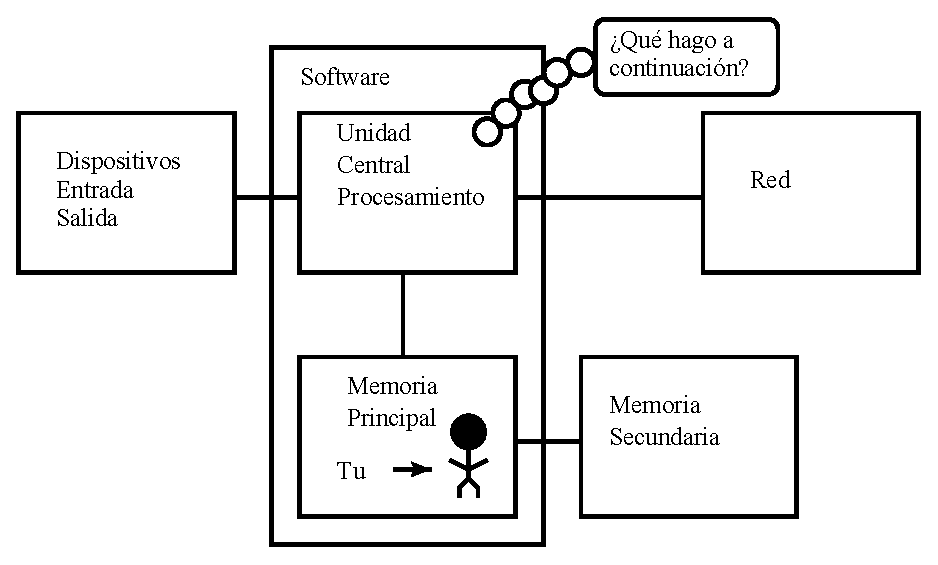
\includegraphics[height=2.50in]{figs2/arch2.eps}}
\afterfig

Tú debes ser la persona que conteste a la pregunta de la CPU ``¿Qué hago a continuación?''.
Pero sería muy incómodo encogerse hasta los 5mm de altura
y meterse dentro del ordenador sólo para poder pasarle un comando
tres mil millones de veces por segundo. Así que en vez de eso,
deberás ponerle por escrito las instrucciones por adelantado.
Llamaremos a esas instrucciones almacenadas un {\bf programa}, y al acto
de escribir las instrucciones y conseguir que
sean correctas, {\bf programar}.

\section{Comprendiendo la programación}

Durante el resto de este libro, intentaremos convertirte en una persona
hábil en el arte de programar. Al final serás un
{\bf programador} --- tal vez no un programador profesional, pero
al menos tendrás la capacidad de echar un vistazo a un problema de análisis
de datos/información y desarrollar un programa para resolverlo.

\index{problem solving}

En cierto sentido, necesitas dos habilidades para ser un programador:

\begin{itemize}

\item En primer lugar, debes dominar el lenguaje de programación (Python) -
debes conocer su vocabulario y su gramática. Debes ser capaz de escribir
las palabras en este nuevo lenguaje correctamente y saber cómo construir
``frases'' bien formadas en este lenguaje.

\item En segundo lugar, debes ``contar una historia''. Al escribir una historia,
combinas palabras y frases para transmitir un concepto al lector.
Son necesarios habilidad y arte para construir la historia, y esa habilidad
se mejora precisamente escribiendo y teniendo cierta retroalimentación.
En programación, nuestro programa es la ``historia'' y el problema
que estás tratando de resolver es el ``concepto''.

\end{itemize}

Una vez que aprendas un lenguaje de programación como Python, encontrarás
mucho más sencillo aprender un segundo lenguaje como JavaScript o C++.
Cada nuevo lenguaje de programación tendrá un vocabulario y gramática muy
diferentes, pero la forma de resolver problemas
va a ser la misma en todos ellos.

Aprenderás el ``vocabulario'' y ``frases'' de Python muy rápidamente.
Te contará un poco más ser capaz de escribir un programa coherente
para resolver un problema nuevo. Se enseña a programar de forma muy similar
a como se enseña a escribir. Se comienza leyendo y explicando programas,
después se escriben programas simples, y se va incrementando la complejidad
de ellos poco a poco. En algún momento ``encuentras tu musa'' y comienzas
a descubrir los patrones por ti mismo, de modo que ya eres capaz de tomar un
problema y escribir un programa para resolverlo. Y una vez has llegado a ese
punto, la programación se convierte en un proceso muy agradable y creativo.

Comenzaremos con el vocabulario y estructura de los programas en Python. Ten
paciencia si la simplicidad de los ejemplos te recuerdan a cuando empezaste
a leer por primera vez.

\section{Palabras y frases}
 \index{programming language}
 \index{language!programming}

A diferencia de los idiomas humanos, el vocabulario de Python es actualmente
bastante reducido. Llamamos a ese ``vocabulario'' las ``palabras reservadas''.
Son palabras que tienen un significado muy especial para Python. Cuando Python
encuentra esas palabras en un programa, tienen un significado y sólo uno para Python.
Más adelante, cuando escribas programas, compondrás tus propias palabras, que tendrán significado para ti, llamadas {\bf variables}. Tendrás una gran libertad para escoger los nombres para tus variables, pero no podrás usar ninguna de las palabras reservadas de Python.

Cuando se entrena a un perro, se usan palabras especiales como
``siéntate'', ``quieto'', y ``traelo''. Cuando hablas con un perro y
no usas ninguna de las palabras reservadas, sólo consigues que te mire
con cara extraña hasta que le digas una palabra reservada.
Por ejemplo, si le dices:
``Me gustaría que hubiera más gente que se dedicase a pasear para mejorar su salud'',
lo que la mayoría de los perros oirían sería:
``bla bla bla {\bf pasear} bla bla bla bla.''.
Esto se debe a que ``pasear'' es una palabra reservada en el idioma del perro.
Mucha gente sugeriría que el idioma entre humanos y gatos no tiene
palabras reservadas\footnote{\url{http://xkcd.com/231/}}.

Las palabras reservadas en el idioma en que los humanos hablan con
Python contiene las siguientes:

\beforeverb
\begin{verbatim}
and       del       from      not       while    
as        elif      global    or        with     
assert    else      if        pass      yield    
break     except    import    print              
class     exec      in        raise              
continue  finally   is        return             
def       for       lambda    try
\end{verbatim}
\afterverb
%
Eso es todo, y a diferencia de un perro, Python ya está completamente entrenado.
Cuando utilices ``try'', Python lo intentará cada vez que se lo digas sin
equivocarse\footnote{``try'' en inglés puede traducirse como ``intento''(N. del Trad.)}.

Aprenderemos esas palabras reservadas y cómo usarlas a su debido tiempo,
pero por ahora nos centraremos en la equivalencia en Python de ``habla''
(en el idioma humano-a-perro). Lo bueno de pedirle a Python que hable
es que podemos incluso decirle qué debe decir, pasándole un mensaje entre comillas:

\beforeverb
\begin{verbatim}
print '¡Hola, mundo!'
\end{verbatim}
\afterverb

Y ya hemos escrito nuestra primera frase sintácticamente correcta en Python.
Nuestra sentencia comienza con la palabra reservada {\bf print}, seguida
por una cadena de texto de nuestra elección, encerrada entre comillas simples.

\section{Conversando con Python}

Ahora que ya conocemos una palabra y una sentencia simple en Python,
debemos aprender cómo comenzar una conversación con Python para probar
nuestras nuevas habilidades.

Antes de que puedas conversar con Python, debes instalar en primer lugar
el software de Python en tu ordenador, y aprender a ponerlo en marcha.
La explicación sobre cómo conseguirlo excede el propósito de este capítulo,
así que te sugiero consultar \url{www.pythonlearn.com}, donde tengo
instrucciones detalladas y capturas de pantallas sobre cómo instalar y poner en marcha
Python en sistemas Macintosh y Windows\footnote{En los capítulos finales del libro también
encontrarás dos apéndices con instrucciones sobre la instalación de Python en esos sistemas (Nota
del trad.)}. En algún momento, terminarás en un terminal
o ventana de comandos, escribirás {\bf python}, y el intérprete de Pyhton
comenzará a ejecutarse en modo interactivo, apareciendo algo como lo siguiente:

\index{interactive mode}

\beforeverb
\begin{verbatim}
Python 2.6.1 (r261:67515, Jun 24 2010, 21:47:49) 
[GCC 4.2.1 (Apple Inc. build 5646)] on darwin
Type "help", "copyright", "credits" or "license" for more information.
>>> 
\end{verbatim}
\afterverb
%
El prompt o indicador {\tt >>>} es el modo que tiene el intérprete de Python de preguntarte:
``¿Qué quieres que haga a continuación?''. Python está preparado para tener una conversación contigo. Todo lo que tienes que hacer es hablar el idioma de Python.

Imaginemos por ejemplo que no conoces ni siquiera la más simple de las palabras o frases del lenguaje Python. Tal vez quieras usar la línea habitual que siguen los astronautas cuando aterrizan en un planeta remoto y quieren hablar con sus habitantes:

\beforeverb
\begin{verbatim}
>>> Venimos en son de paz, por favor llevadnos ante vuestro lider
  File "<stdin>", line 1
    Venimos en son de paz, por favor llevadnos ante vuestro lider
         ^
SyntaxError: invalid syntax
>>> 
\end{verbatim}
\afterverb
%
Esto no está funcionando. A menos que pienses en algo rápido,
los habitantes del planeta probablemente te clavarán sus lanzas,
te ensartarán en un asador, te cocinarán sobre el fuego, y te usarán como cena.

Por suerte has comprado una copia de este libro durante el viaje, así que lo hojeas
hasta llegar precisamente a esta página y pruebas de nuevo:

\beforeverb
\begin{verbatim}
>>> print '¡Hola, mundo!'
¡Hola, mundo!
\end{verbatim}
\afterverb
%
Esto tiene mejor aspecto, así que intentas comunicarte un poco
más:

\beforeverb
\begin{verbatim}
>>> print 'Tú debes ser el dios legendario que viene del cielo'
Tú debes ser el dios legendario que viene del cielo
>>> print 'Hemos estado esperándote durante mucho tiempo'
Hemos estado esperándote durante mucho tiempo
>>> print 'Nuestras leyendas dicen que debes estar muy sabroso con mostaza'
Nuestras leyendas dicen que debes estar muy sabroso con mostaza
>>> print 'Vamos a tener un festín esta noche a menos que digas
  File "<stdin>", line 1
    print 'Vamos a tener un festín esta noche a menos que digas
                                                              ^
SyntaxError: EOL while scanning string literal
>>> 
\end{verbatim}
\afterverb
%
La conversación fue bien durante un rato, y entonces, en cuanto
cometiste un pequeño error usando el lenguaje Python, Python
volvió a apuntarte con las lanzas.

En este momento, ya deberías haberte dado cuenta de que, a pesar de que Python
es increíblemente complejo, potente y muy exigente con
la sintaxis que debes usar para comunicarte con él, Python {\em no} es
inteligente. En realidad tan sólo estás teniendo una conversación
contigo mismo, eso sí, usando una sintaxis correcta.

En cierto sentido, cuando usas un programa escrito por otra persona,
la conversación se mantiene entre tú mismo y esos otros programadores,
con Python actuando como intermediario. Python es un
modo de que los creadores de programas puedan expresar cómo creen
que deben desarrollarse las conversaciones. Y dentro
de unos pocos capítulos más, tú serás uno de esos programadores
que usan Python para hablar con los usuarios de sus programas.

Antes de terminar nuestra primera conversación con el intérprete
de Python, probablemente debas saber cual es el modo correcto
de decir ``adios'' cuando estás interactuando con los
habitantes del Planeta Python:

\beforeverb
\begin{verbatim}
>>> adios
Traceback (most recent call last):
  File "<stdin>", line 1, in <module>
NameError: name 'adios' is not defined

>>> if you don't mind, I need to leave
  File "<stdin>", line 1
    if you don't mind, I need to leave
             ^
SyntaxError: invalid syntax

>>> quit()
\end{verbatim}
\afterverb
%
Te habrás dado cuenta de que el error es diferente en los primeros
dos intentos, a pesar de ser ambos incorrectos. El segundo error es diferente porque
{\bf if} es una palabra reservada, y Python vió la palabra
reservada en la frase y creyó que estabas intentando decirle algo, pero encontró
la sintaxis de la sentencia incorrecta.

El modo correcto de decir ``adios'' a Python es introducir
{\bf quit()} en el indicador interactivo {\tt >>>}.
Probablemente te hubiera llevado un buen rato adivinarlo,
así que es posible que tener un libro a mano
esté empezando a resultarte útil.

\section{Terminología: intérprete y compilador}

Python es un lenguaje de {\bf alto nivel}, que intenta ser relativamente
sencillo de escribir y leer para los humanos y fácil de leer y procesar para
los ordenadores. Hay otros lenguajes de alto nivel, como Java, C++,
PHP, Ruby, Basic, Perl, JavaScript, y muchos más. El hardware que está
actualmente dentro del la Unidad Central de Procesamiento (CPU) no comprende
ninguno de estos lenguajes de alto nivel.

La CPU comprende un lenguaje que se llama {\bf código máquina}. El código
máquina es muy simple y francamente muy cansado de escribir, porque
en él todo está representado por ceros y unos:

\beforeverb
\begin{verbatim}
01010001110100100101010000001111
11100110000011101010010101101101
...
\end{verbatim}
\afterverb
%
El código máquina superficialmente parece muy sencillo, dado que sólo hay
ceros y unos, pero su sintaxis es incluso más complicada
y mucho más intrincada que Python. Así que muy pocos programadores
usan este lenguaje. En vez de eso, se han construido varios traductores para
permitir a los programadores escribir en lenguajes de alto nivel, como Python
o JavaScript, y esos traductores convierten luego los programas a código máquina
para que la CPU pueda ejecutarlos.

Dado que el código máquina está ligado al hardware del ordenador, ese código
no es {\bf portable} a través de los diferentes tipos de hardware. Los programas escritos
en lenguajes de alto nivel pueden ser trasladados entre ordenadores diferentes usando
un intérprete diferente en la nueva máquina o recompilando el código para crear
una versión en código máquina del programa para el nuevo equipo.

Estos traductores de lenguajes de programación se clasifican en dos categorías generales:
(1) intérpretes y (2) compiladores.

Un {\bf intérprete} lee el código fuente del programa tal y como lo ha escrito
el programador, analiza ese código fuente e interpreta las instrucciones al vuelo.
Python es un intérprete y cuando estamos haciéndolo funcionar de forma interactiva,
podemos escribir una línea de Python (una sentencia), y Python la procesa inmediatamente
y queda listo para que podemos escribir otra nueva línea.

Algunas de las líneas de Python le indican que lo que queremos es recordar cierto
valor para más tarde. Debemos elegir un nombre para que ese valor sea recordado y
podremos usar ese nombre simbólico para recuperar el valor después. Usamos el
término {\bf variable} para referirnos a las etiquetas que utilizamos para manejar esos
datos almacenados.

\beforeverb
\begin{verbatim}
>>> x = 6
>>> print x
6
>>> y = x * 7
>>> print y
42
>>> 
\end{verbatim}
\afterverb
%
En este ejemplo, le pedimos a Python que recuerde el valor seis y use la etiqueta {\bf x},
para que podemos recuperar ese valor más tarde. Comprobamos que Python ha guardado de
momento el valor usando {\bf print}. A continuación le pedimos a Python que recupere {\bf x}, lo multiplique por siete y coloque el nuevo valor calculado en {\bf y}. Finalmente, le pedimos a Python que imprima el valor que está actualmente en {\bf y}.

Aunque estemos escribiendo estos comandos en Python línea por línea, Python
los está tratando como una secuencia ordenada de declaraciones, de modo
que las últimas declaraciones son capaces de recuperar datos creados en las
anteriores. Estamos escribiendo nuestro primer párrafo simple con cuatro frases
en un orden lógico y útil.

La naturaleza de un {\bf intérprete} es ser capaz de tener una conversación interactiva como se muestra más arriba. Un {\bf compilador} necesita que le entreguen el programa
completo en un archivo, y después
ejecuta un proceso para trasladar el código fuente de alto nivel a código máquina.
A continuación el compilador guarda el código máquina resultante en un archivo para su
posterior ejecución. 

Si usas un sistema Windows, a menudo esos programas ejecutables en código máquina tienen un sufijo como ``.exe'' or ``.dll'', que indican ``executable (ejecutable)'' y ``dynamic
link library (librería de enlace dinámico)'' respectivamente. En Linux y Macintosh
no hay un sufijo que marque de forma única un archivo como ejecutable.

Si abrieras un archivo ejecutable en un editor de texto, se mostraría algo
completamente disparatado e ilegible:

\beforeverb
\begin{verbatim}
^?ELF^A^A^A^@^@^@^@^@^@^@^@^@^B^@^C^@^A^@^@^@\xa0\x82
^D^H4^@^@^@\x90^]^@^@^@^@^@^@4^@ ^@^G^@(^@$^@!^@^F^@
^@^@4^@^@^@4\x80^D^H4\x80^D^H\xe0^@^@^@\xe0^@^@^@^E
^@^@^@^D^@^@^@^C^@^@^@^T^A^@^@^T\x81^D^H^T\x81^D^H^S
^@^@^@^S^@^@^@^D^@^@^@^A^@^@^@^A\^D^HQVhT\x83^D^H\xe8
....
\end{verbatim}
\afterverb
%
No es fácil leer o escribir código máquina, así que está bien que tengamos
{\bf intérpretes} y {\bf compiladores} que nos permitan escribir en lenguajes
de alto nivel, como Python o C.

En este momento de la discusión acerca de compiladores e intérpretes, deberías
estar preguntándote algunas cosas sobre el mismo intérprete de Python. ¿En qué
lenguaje ha sido escrito? ¿Ha sido escrito en un lenguaje compilado? Cuando escribimos ``python'', ¿qué es exactamente lo que ocurre?

El intérprete de Python está escrito en un lenguaje de alto nivel llamado ``C''.
Puedes ver el código fuente real del intérprete de Python acudiendo a
\url{www.python.org}, y hacer lo que quieras con su código fuente.
Así que el propio Python es también un programa, y está compilado en código máquina.
Cuando instalaste Python en tu ordenador (o el vendedor lo instaló),
pusiste una copia del código máquina del programa Python traducido para tu sistema.
En Windows, el ejecutable en código máquina del propio Python es probablemente
un archivo con un nombre como:

\beforeverb
\begin{verbatim}
C:\Python27\python.exe
\end{verbatim}
\afterverb
%
Esto ya es más de lo que en realidad necesitas saber para ser un programador en Python,
pero a veces es mejor responder a estas típicas preguntillas justo
al principio.

\section{Escribir un programa}

Escribir frases en el intérprete de Python es un buen modo de experimentar
con las características de Python, pero no se recomienda para resolver problemas
de cierta complejidad.

Cuando queremos escribir un programa,
usamos un editor de texto para escribir las instrucciones de Python en un archivo,
que se denomina un {\bf script}. Por
convención, los scripts en Python tienen nombres que terminan en {\tt .py}.

\index{script}

Para ejecutar un script, tienes que indicarle al intérprete de Python
el nombre del archivo. En una ventana de comandos de Unix o Windows,
puedes escribir {\tt python hello.py} así:

\beforeverb
\begin{verbatim}
csev$ cat hello.py
print '¡Hola, mundo!'
csev$ python hello.py
¡Hola, mundo!
csev$
\end{verbatim}
\afterverb
%
El ``csev\$'' es el indicador del sistema operativo, y el ``cat hello.py'' nos
está mostrando que el archivo ``hello.py'' contiene un programa Python de una línea
que imprime una cadena.

Estamos llamando al intérprete de Pyhton e indicándole que lea el código fuente del
archivo ``hello.py'', en vez de ir escribiendo nosotros las líneas de código Python
de forma interactiva.

Habrás notado que no es necesario poner {\\bf quit()} al final del programa
Python en el archivo. Cuando Python está leyendo el código fuente
desde un archivo, sabe parar cuando llega al final del fichero.

\section{¿Qué es un programa?}

La definición más básica de un {\bf programa} es que se trata de una
secuencia de sentencias de Python que han sido creadas para hacer algo.
Incluso nuestro simple script {\bf hello.py} es un programa. Es un programa
de una sola línea y no particularmente útil, pero en su más estricta definición,
es un programa Python. 

Debería ser más sencillo comprender qué es un programa si pensásemos en un problema
que pudiera resolverse mediante programación, y a continuación estudiásemos cómo sería el
programa que resolviera ese problema.

Imaginemos que estás haciendo una investigación sobre estadística social en los mensajes
de Facebook, y estás interesado en saber cuál es la palabra que se usa con mayor frecuencia
en una serie de mensajes. Podrías imprimir la cadena de mensajes de Facebook y estudiar
detenidamente el texto, buscando la palabra más común, pero eso te llevaría mucho tiempo
y lo más probable sería que cometieses errores. Sería más inteligente escribir un programa
en Python para realizar la tarea rápidamente y con precisión, y así podrías emplear el fin
de semana en hacer algo divertido.

Por ejemplo, mira el texto siguiente acerca de un payaso y un coche. Fijate en el
texto y busca cual es la palabra más común y cuántas veces se repite.

\beforeverb
\begin{verbatim}
el payaso corrió detrás del coche y el coche se metió en la carpa
y la carpa se cayó sobre el payaso y el coche
\end{verbatim}
\afterverb
%
Después imagina que estás haciendo esta tarea buscando en millones de líneas de
texto. Francamente, te resultaría más rápido aprender Python y escribir un
programa para contar las palabras que revisarlas manualmente una a una.

La buena noticia es que a mí ya se me ha ocurrido un programa
simple para encontrar la palabra más común en un archivo de texto. Lo he escrito,
probado, y ahora te lo doy a ti para que lo uses y puedas ahorrarte algo de tiempo.

\beforeverb
\begin{verbatim}
name = raw_input('Introduce archivo:')
manejador = open(nombre, 'r')
texto = manejador.read()
palabras = texto.split()
contadores = dict()

for palabra in palabras:
   contadores[palabra] = contadores.get(palabra,0) + 1

mayorcantidad = None
mayorpalabra = None
for palabra,contador in contadores.items():
    if mayorcantidad is None or contador > mayorcantidad:
        mayorpalabra = palabra
        mayorcantidad = contador

print mayorpalabra, mayorcantidad
\end{verbatim}
\afterverb
%
No necesitas ni siquiera saber Python para utilizar este programa. Deberás llegar hasta
el capítulo 10 de este libro para comprender del todo las impresionantes técnicas que
se han usado para crear este programa. Eres el usuario final, simplemente utiliza el
programa y maravíllate de su ingenio y de cuánto esfuerzo manual te ha ahorrado.
Simplemente escribe el código
en un archivo llamado {\bf words.py} y ejecútalo, o descarga el código fuente
de \url{http://www.pythonlearn.com/code/} y hazlo funcionar.

\index{program}
Este es un buen ejemplo de cómo Python y el lenguaje Python están actuando de
intermediarios entre tú (el usuario final) y yo (el programador). Python es para nosotros
un modo de intercambiar secuencias de instrucciones útiles (p.e. programas) en un
lenguaje común que puede ser usado por cualquiera que instale
Python en su ordenador. Así que ninguno de nosotros estamos hablando {\em a Python},
sino que estamos comunicándonos mutuamente {\em a través de} Python.

\section{Los bloques de construcción de los programas}

En los próximos capítulos, aprenderemos más acerca del vocabulario, estructura de las
frases, estructura de los párrafos, y estructura de las historias de Python. Aprenderemos
sobre las potentes capacidades de Python y cómo usar esas capacidades juntas para crear
programas útiles.

Hay ciertos modelos conceptuales de bajo nivel que se usan para construir programas.
Estas estructuras no son exclusivas de los programas Python, sino que son parte de
cualquier lenguaje de programación, desde el código máquina hasta los lenguajes de alto
nivel.

\begin{description}

\item[entrada:] Obtiene datos del ``mundo exterior''. Puede consistir en
leer datos de un archivo, o incluso de algún tipo de sensor, como un micrófono
o GPS. En nuestros programas iniciales la entrada vendrá del propio usuario,
escribiendo datos en el teclado.

\item[salida:] Muestra el resultado del programa en la pantalla
o lo almacena en un archivo; o tal vez lo escribe en un dispositivo, como puede ser
un altavoz, para reproducir música o leer texto.

\item[ejecución secuencial:] Ejecuta sentencias una detrás de otra,
en el orden en que se encuentran en el script.

\item[ejecución condicional:] Comprueba ciertas condiciones y
después ejecuta u omite una secuencia de sentencias.

\item[ejecución repetida:] Ejecuta cierto conjunto de sentencias
repetidamente, normalmente con alguna variación.

\item[reutilización:] Se escriben un conjunto de instrucciones una vez y se las da un nombre
para después reutilizarlas cuando sean necesarias en cualquier otra parte
del programa.

\end{description}

Parece demasiado simple para ser verdad, y por supuesto nunca es tan simple.
Es como decir que caminar es simplemente
``poner un pie delante del otro''. El ``arte''
de escribir un programa es componer y entrelazar juntos estos
elementos básicos muchas veces, para producir algo
que sea útil a sus usuarios.

El programa anterior que calcula el número de palabras usa directamente
todos estos patrones, excepto uno.

\section{¿Qué es posible que vaya mal?}

Como hemos visto en nuestra primera conversación con Python, deberemos
comunicarnos de forma muy precisa cuando escribamos código Python. La mínima
desviación o error provocará que Python deje de ejecutar
nuestro programa.

Los programadores novatos a menudo se toman el hecho de que Python no
deje espacio para errores como una prueba de que Python es perverso, odioso y cruel.
Aunque a Python parece que le gustan todos los demás, reconoce a los novatos
y les guarda rencor. Debido a ese rencor,
Python toma sus programas perfectamente escritos y los rechaza como si fueran
``inútiles'' sólo para atormentarnos.

\beforeverb
\begin{verbatim}
>>> primt '¡Hola, mundo!'
  File "<stdin>", line 1
    primt '¡Hola, mundo!'
                       ^
SyntaxError: invalid syntax
>>> primt 'Hola, mundo'
  File "<stdin>", line 1
    primt 'Hola, mundo'
                      ^
SyntaxError: invalid syntax
>>> ¡Te odio, Python!
  File "<stdin>", line 1
    ¡Te odio, Python!
         ^
SyntaxError: invalid syntax
>>> si sales fuera, te daré una lección
  File "<stdin>", line 1
    si sales fuera, te daré una lección
              ^
SyntaxError: invalid syntax
>>> 
\end{verbatim}
\afterverb
%
Hay poco que ganar discutiendo con Python. Sólo es una herramienta.
No tiene emociones, es feliz y está listo para servirte en cualquier momento
que le necesites. Sus mensajes de error parecen crueles, pero son simples
peticiones de ayuda de Python. Ha examinado lo que has escrito y simplemente
no es capaz de entender lo que has puesto.

Python se parece mucho a un perro: te quiere incondicionalmente, pero sólo es capaz
de entender unas pocas palabras clave, así que te mira con una expresión
adorable en su cara ({\tt >>>}),y espera a que tú le digas algo que él pueda comprender.
Cuando Python dice ``SyntaxError: invalid syntax'', está simplemente agitando
su cola y diciendo: ``Me parece que has dicho algo, pero es que no comprendo
lo que significa. De todos modos, sigue hablando conmigo, por favor ({\tt >>>}).''

Cuando tus programas vayan aumentando su complejidad, te encontrarás con
tres tipos de errores en general:

\begin{description}

\item[Errores de sintaxis:] Estos son los primeros errores que cometerás y los más
fáciles de corregir. Un error de sintaxis quiere decir que has violado las reglas de la
``gramática'' de Python. Python hace lo que puede para indicar la línea y el carácter
correctos en donde ha cree que está la confusión. Lo único complicado de los errores de
sintaxis es que a veces el error que se necesita corregir está en alguna línea del
programa anterior a aquella en la cual Python emite el {\em aviso}. De modo que la línea
y el carácter que Python indica en un error de sintaxis pueden ser sólo un punto de
partida para tu investigación.  

\item[Errores lógicos:] Un error lógico es cuando tu programa tiene una sintaxis correcta,
pero existe un error en el orden de las sentencias o tal vez un error en cómo las
sentencias se relacionan unas con otras.
Un buen ejemplo de un error lógico sería, ``toma un trago de tu botella de agua, ponla
en tu mochila, camina hasta la biblioteca, y luego vuelve a poner el tapón a la botella.'' 

\item[Errores semánticos:] Un error semántico se produce cuando la descripción de los
pasos a seguir es sintácticamente perfecta y se realiza en el orden correcto, pero
simplemente existe un error en el programa. El programa es perfectamente correcto, pero
no realiza aquello que tú {\em pretendías} que hiciera. Un ejemplo sencillo podría ser
si tú estuvieses indicando a alguien el camino hacia un restaurante y dijeras:
``...cuando llegues a la intersección con la gasolinera, gira a la izquierda, continúa
durante kilómetro y medio y el edificio rojo de tu derecha será el restaurante.'' Tu amigo
se retrasará y te llamará para decirte que está en una granja, y dando vueltas alrededor
de un granero, sin que haya señal alguna de un restaurante.
Entonces le preguntarás: ``¿Giraste a la izquierda o a la derecha en la gasolinera?'', y él
responderá: ``Seguí al pie de la letra tus indicaciones, las tengo por escrito, y decían
que debía girar la izquierda y continuar kilómetro y medio desde la gasolinera.'' Entonces
le dirás: ``Lo siento mucho, porque aunque mis instrucciones son sintácticamente
correctas, por desgracia contienen un pequeño e indetectado error semántico.''.

\end{description}

Cuando se produce cualquiera de los tres tipos de errores, Python de nuevo está
simplemente intentando por todos los medios hacer exactamente lo que tú le has pedido.

\section{El viaje de aprendizaje}

Según vayas avanzando por el resto del libro, no te asustes si los conceptos
no parecen encajar bien unos con otros al principio. Cuando estabas aprendiendo a hablar,
no supuso un problema que durante los primeros años sólo pudieras emitir lindos
balbuceos. Y también fue normal que te llevara seis meses pasar de un vocabulario simple
a frases simples y que te llevara 5-6 años más pasar de frases a párrafos, y unos cuantos
años más hasta que fuiste capaz de escribir una historia corta interesante por ti mismo.

Pretendemos que aprendas Python mucho más rápidamente, y todo al mismo tiempo
durante los próximos capítulos.
Aún así, ten en cuenta que esto es como un aprender un idioma nuevo, que lleva un tiempo
absorber y comprender antes de que te resulte familiar.
Eso produce cierta confusión, ya que visitaremos y volveremos a visitar
temas para intentar que consigas ver el conjunto del cuadro mientras vamos definiendo
los pequeños fragmentos que forman esa obra completa. A pesar de que el libro está
escrito de forma lineal, y que si estás participando en un curso éste también avanzará
de forma lineal, no dudes en ser no lineal en el modo en que te aproximes al material.
Avanza y retrocede y lee a veces por encima. Al ojear material más avanzado sin comprender del
todo los detalles tendrás una mejor comprensión del ``¿por qué?'' de la programación.
Al revisar el material anterior e incluso al rehacer los ejercicios previos,
te darás cuenta que ya has aprendido un montón de materia, incluso si la materia
sobre la que estás trabajando en ese momento parece un poco impenetrable.

Normalmente, cuando uno aprende su primer lenguaje de programación, hay unos pocos
momentos estupendos ``¡A-já!'', en los cuales puedes levantar la vista de la roca que
estás machacando con martillo y cincel, separarte unos pasos y comprobar
que lo que estás intentando construir es una maravillosa escultura.

Si algo parece particularmente difícil, generalmente no vale la pena quedarse mirándolo
toda la noche. Tómate un respiro, échate una siesta, come algo, explícale a alguien
(quizás a tu perro) con qué estás teniendo problemas, y después vuelve a ello con nuevos
ojos. Te aseguro que una vez que aprendas los conceptos de la programación en
el libro, volverás atrás y verás que en realidad todo era fácil y elegante y que
simplemente te ha llevado un poco de tiempo llegar a absorberlo.

\section{Glosario}

\begin{description}

\item[bug:] Un error en un programa.
\index{bug}

\item[código fuente:] Un programa en un lenguaje de alto nivel.
\index{source code}

\item[código máquina:] El lenguaje de más bajo nivel para el software, ya que se trata
del lenguaje que es directamente ejecutado por la unidad central de procesamiento
(CPU).
\index{machine code}

\item[compilar:] Traducir un programa escrito en un lenguaje de alto nivel
a otro lenguaje de bajo nivel de una vez, preparándolo para su posterior
ejecución.
\index{compile}

\item[error semántico:] Un error en un programa que provoca que haga algo
distinto de lo que el programador pretendía.
\index{semantic error}

\item[interpretar:]  Ejecutar un programa en un lenguaje de alto nivel
traduciendo sus líneas de una en una.
\index{interpret}

\item[lenguaje de alto nivel:]  Un lenguaje de programación como Python, que
está diseñado para ser sencillo de leer y escribir para los humanos.
\index{high-level language}

\item[lenguaje de bajo nivel:]  Un lenguaje de programación que ha sido diseñado
para ser sencillo de ejecutar para un ordenador; también se le llama ``código máquina''
o ``lenguaje ensamblador''.
\index{low-level language}

\item[memoria principal:] Almacena programas y datos. La memoria principal pierde
su información cuando se interrumpe la energía que la alimenta.
\index{main memory}

\item[memoria secundaria:] Almacena programas y datos y retienen su
información incluso cuando la corriente se interrumpe. Generalmente es más lenta
que la memoria principal. Ejemplos de memoria secundaria pueden ser unidades de
disco y memorias flash en lápices USB.
\index{secondary memory}

\item[modo interactivo:] Un modo de uso de usar el intérprete de Python
escribiendo comandos y expresiones en el prompt (indicador).
\index{interactive mode}

\item[parsear:] Examinar un programa y analizar su estructura sintáctica.
\index{parse}

\item[portabilidad:]  La propiedad de un programa que le permite funcionar en más
de un tipo de ordenador.
\index{portability}

\item[programa:] Un conjunto de instrucciones que especifican un cálculo.
\index{program}

\item[prompt:] Cuando un programa muestra un mensaje y se detiene para que
el usuario escriba alguna entrada para el programa.
\index{prompt}

\item[resolución de problemas:]  El proceso de formular un problema, encontrar
una solución y expresar la solución.
\index{problem solving}

\item[semántica:] El significado de un programa.
\index{semantics}

\item[sentencia print:]  Una instrucción que provoca que el intérprete de Python
muestre un valor en la pantalla.
\index{print statement}
\index{statement!print}

\item[unidad central de procesamiento:] El corazón de cualquier ordenador. Es lo que
ejecuta el software que escribimos; también se le suele llamar ``CPU'' o ``el procesador''.
\index{central processing unit}
\index{CPU}

\end{description}

\section{Ejercicios}


\begin{ex}
¿Cuál es la función de la memoria secundaria en un ordenador?

a) Ejecutar todos los cálculos y lógica del programa\\
b) Recuperar páginas web de Internet\\
c) Almacenar información durante mucho tiempo -- incluso entre ciclos de apagado-encendido\\
d) Recoger la entrada del usuario
\end{ex}

\begin{ex}
¿Qué es un programa?
\end{ex}

\begin{ex}
¿Cuál es la diferencia entre un compilador y un intérprete?
\end{ex}

\begin{ex}
¿Cuál de los siguientes contiene ``código máquina''?

a) El intérprete de Python\\
b) El teclado\\
c) El código fuente de Python\\
d) Un documento de un procesador de texto
\end{ex}

\begin{ex}
¿Qué está mal en el código siguiente?:

\beforeverb
\begin{verbatim}
>>> primt '¡Hola, mundo!'
  File "<stdin>", line 1
    primt '¡Hola, mundo!'
                       ^
SyntaxError: invalid syntax
>>> 
\end{verbatim}
\afterverb

\end{ex}

\begin{ex}
¿En qué parte del ordenador queda almacenada una variable como ``X''
después de que termine la siguiente línea de Python?:

\beforeverb
\begin{verbatim}
x = 123
\end{verbatim}
\afterverb
%
a) Unidad Central de Procesamiento\\
b) Memoria Principal\\
c) Memoria Secundaria\\
d) Dispositivos de Entrada\\
e) Dispositivos de Salida
\end{ex}

\begin{ex}
¿Qué imprimirá en pantalla el siguiente programa?:

\beforeverb
\begin{verbatim}
x = 43
x = x + 1
print x
\end{verbatim}
\afterverb
%
a) 43\\
b) 44\\
c) x + 1\\
d) Error, porque x = x + 1 no es posible matemáticamente
\end{ex}

\begin{ex}
Explica cada uno de los siguientes conceptos usando como ejemplo una capacidad humana:
(1) Unidad Central de Procesamiento, (2) Memoria Principal, (3) Memoria Secundaria, 
(4) Dispositivo de Entrada, y
(5) Dispositivo de Salida.
Por ejemplo, ``¿Cuál es el equivalente humano a la Unidad Central de Procesamiento''? 
\end{ex}

\begin{ex}
¿Cómo puedes corregir un ``Error de sintaxis''?
\end{ex}

